\documentclass{beamer}
\usetheme{CambridgeUS}
\usepackage[spanish]{babel}
\usepackage[utf8]{inputenc}
\usefonttheme{professionalfonts}
\usepackage{times}
\usepackage{tikz}
\usepackage{amsmath}
\usepackage{mathrsfs}       %negrita en ecuaciones
\usepackage{upgreek}        %negrita en letras griegas
\usepackage{verbatim}
\usetikzlibrary{arrows,shapes}
\usepackage{graphicx}
\usepackage{subfigure}
\usepackage{bibentry}
\graphicspath{{imagenes/}}

\author{Daniel Villarreal}
\title{Sustentación de Trabajo de Grado}

%funciones creadas
\newcommand{\negd}[1]{\mathbf{#1}}    %negrita letras normales
\newcommand{\neggr}[1]{\boldsymbol{#1}}

\begin{document}

%página 1
\begin{frame}
     \frametitle{Estimación de la Irradiancia Solar en la República de Panamá}
     %\framesubtitle{Asesor: Dr. Abdoulaye Diallo, Estudiante: Daniel Villarreal}
      \begin{figure}[h!]
         \centering \subfigure{
\includegraphics[width=2cm, height=0.7cm]{logo_utp}}
         \hspace{5cm}
         \centering \subfigure{
\includegraphics[width=3cm, height=0.3cm]{senacyt}}
      \end{figure}
      \begin{center}
         {\scshape \small Universidad Tecnológica de Panamá \par}
         {\scshape Facultad de Ciencias y Tecnología \par}
         {\scshape Maestría en Ciencias Físicas \par}
         \vspace{0.3cm}
         Presentado por: \\
         Daniel Villarreal Chiari \\
         \begin{large}
            Asesor: \\
            Abdoulaye F. Diallo \\
         \end{large}
      \end{center}
\end{frame}

%página 2
\begin{frame}
    \frametitle{Contenido}
    \tableofcontents
\end{frame}

%página 3
\section{La Radiación Solar}
\begin{frame}
   \frametitle{La Radiación Solar}
   \begin{figure}[h!]
   \begin{minipage}{0.3\textwidth}
   \begin{flushleft}
   \begin{itemize}
      \item\small En el Sol, ocurren reacciones nucleares, que dependen de sus características estructurales. 
      \item\small Los fotones resultantes de estas reacciones nucleares transportan la energía producida. 
   \end{itemize}
   \end{flushleft} 
   \end{minipage}
   \begin{minipage}{0.5\textwidth}
      \centering 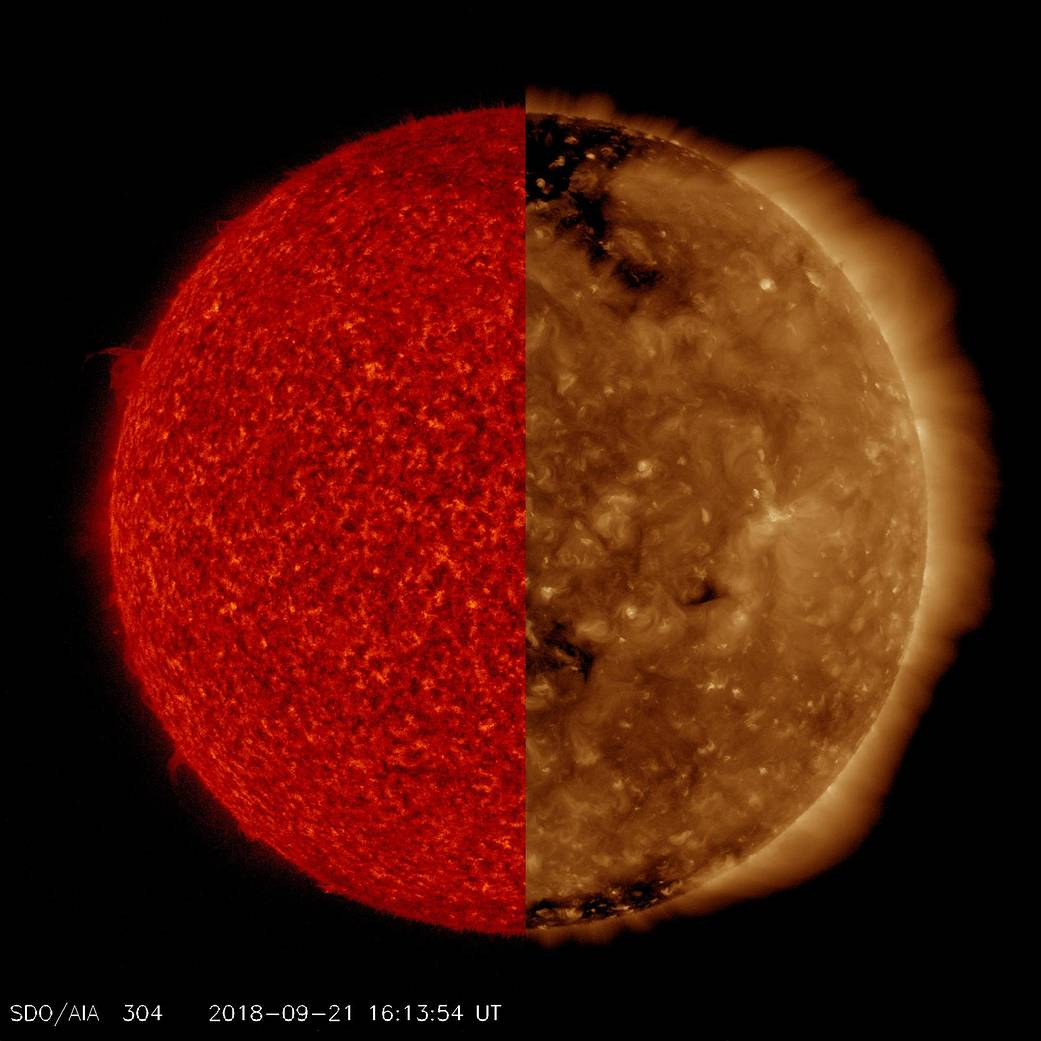
\includegraphics[width=4.5cm, height=4.5cm]{radiacion_solar}
      \caption{\tiny Imagen del Sol en ultravioleta (izq.) e infrarojo (der.). Fuente: NASA/GSFC/Solar Dynamics Observatory}
   \end{minipage}
   \end{figure}
\end{frame}



\end{document}
